% main.tex
% The Evolutionary Map of the Entire Universe
% Self-contained LaTeX project, standard article class
% Compile with: xelatex -> biber -> xelatex -> xelatex
% Or:         pdflatex -> biber -> pdflatex -> pdflatex

\documentclass[a4paper,11pt]{article}

% Encoding & fonts
\usepackage[utf8]{inputenc}
\usepackage[T1]{fontenc}
\usepackage{lmodern}
\usepackage{microtype}

% Math
\usepackage{amsmath,amssymb,amsfonts,amsthm}

% Figures & plotting
\usepackage{graphicx}
\usepackage{tikz}
\usepackage{pgfplots}
\pgfplotsset{compat=1.18}
\usetikzlibrary{shapes,arrows,positioning,calc}

% Tables & lists
\usepackage{booktabs}
\usepackage{enumitem}
\usepackage{array}

% Bibliography
\usepackage[
    backend=biber,
    style=numeric,
    sorting=none,
    citestyle=numeric,
    maxbibnames=99,
    giveninits=true,
    doi=false,
    isbn=false,
    url=false,
    eprint=false
]{biblatex}
\addbibresource{references.bib}

% Hyperlinks
\usepackage{xcolor}
\usepackage{hyperref}
\hypersetup{
    colorlinks=true,
    linkcolor=blue!70!black,
    citecolor=blue!70!black,
    urlcolor=magenta!70!black,
    pdftitle={The Evolutionary Map of the Entire Universe},
    pdfauthor={Xiaohui Li}
}

% Layout
\usepackage{geometry}
\geometry{left=2.5cm,right=2.5cm,top=2.5cm,bottom=2.5cm}
\usepackage{setspace}
\onehalfspacing
\usepackage{titlesec}
\titleformat{\section}{\large\bfseries}{\thesection}{1em}{}
\titleformat{\subsection}{\normalsize\bfseries}{\thesubsection}{1em}{}

% Caption
\usepackage{caption}
\captionsetup{font=small,labelfont=bf}

% Custom commands
\newcommand{\LCDM}{$\Lambda$CDM}
\newcommand{\CCCM}{CCCM}

\title{\bfseries The Evolutionary Map of the Entire Universe:\\
A Chiral Cyclic Cosmological Framework}

\author{
    Xiaohui Li\\
    \small Independent Researcher, Baoji, China\\
    \small ORCID: 0009-0003-8233-7191\\
    \small Correspondence: \href{mailto:danceluck@163.com}{danceluck@163.com}
}

\date{}

\begin{document}

\maketitle

\begin{abstract}
\noindent
We propose a conceptual framework, termed the Chiral Cyclic Cosmological Model (\CCCM), that synthesizes time-symmetric evolution, cosmic expansion--contraction cycles, and quantum chirality into a coherent narrative for the origin, evolution, and fate of the Universe. In this model, the Big Bang is interpreted as a chirality-symmetric repulsive phase; the subsequent transition to a marginally chiral dominance drives gravitational aggregation, structure formation, and the emergence of biological homochirality; and the terminal high-order, low-entropy state---operationally defined as the ``Great Refinement''---produces primordial seeds that may manifest as black holes, each potentially hosting a nested internal universe. We derive a set of falsifiable predictions: (i) a measurable excess of one quantum chirality in the early Universe correlated with baryon asymmetry; (ii) an early black-hole seed mass function extending above standard Population-III stellar-remnant expectations; and (iii) a stochastic gravitational-wave background with a characteristic chirality-dependent polarization signature. We place these predictions in the context of current data from the Planck satellite, JWST high-redshift quasar observations, and LIGO/Virgo/KAGRA gravitational-wave catalogues. The model is presented as a hypothesis requiring rigorous observational and numerical tests rather than an established theory.
\end{abstract}

\noindent\textbf{Keywords:} cosmology; quantum chirality; cyclic universe; black-hole seeds; baryon asymmetry; entropy reversal; early Universe; gravitational waves

\section{Introduction}
\label{sec:intro}

Contemporary cosmology rests on three empirical pillars: the cosmic microwave background (CMB)~\cite{Planck2018}, the accelerating expansion inferred from Type Ia supernovae~\cite{Riess1998}, and the large-scale distribution of galaxies~\cite{Abazajian2005}. These observations are elegantly accommodated by the \LCDM{} model, which posits an early inflationary epoch, a composition dominated by dark energy ($\Lambda$) and cold dark matter (CDM), and a flat spatial geometry~\cite{Peebles2020}. Nevertheless, \LCDM{} leaves several foundational questions open: the nature of dark energy, the origin of the Big Bang singularity, the mechanism of baryogenesis, and the arrow of time~\cite{Carroll2010}.

A recurring motif in attempts to address these questions is the idea of a cyclic or oscillating universe~\cite{Steinhardt2002,Penrose2010}. Separately, the observed homochirality of biological molecules and the chiral asymmetry of the weak interaction suggest that ``handedness'' may be a deep feature of nature rather than a biological accident~\cite{Glashow1961,Hazen2007}. Here we propose the Chiral Cyclic Cosmological Model (\CCCM), a speculative but systematically stated framework in which quantum chirality is the driver of transitions between the principal epochs of cosmic history.

The \CCCM{} consists of five linked propositions:
\begin{enumerate}[label=(\arabic*)]
    \item The Universe begins in a maximally symmetric ``seed'' state with equal abundances of left- and right-handed quantum modes.
    \item The initial expansion is effectively repulsive because opposite chiralities are mutually excluded.
    \item A stochastic fluctuation produces a slight excess of one chirality; this tiny bias amplifies, converting repulsion into attraction and triggering structure formation.
    \item Gravitational collapse, life, and intelligence are stages in an entropy-reversing march toward a ``Great Refinement''---a globally ordered, low-entropy terminal state.
    \item The terminal state produces new seeds, plausibly identified with black holes, each containing a nested universe, thereby closing the cycle.
\end{enumerate}

We emphasize that propositions (4) and (5) are theoretical extensions; they are not validated by existing data. The value of the \CCCM{} lies in its capacity to generate falsifiable predictions that can be confronted with current and future observations.

\section{Theoretical Framework}
\label{sec:theory}

\subsection{Chirality as a cosmological order parameter}

In particle physics, chirality is a Lorentz-invariant property of massless fermions; the weak interaction violates parity and couples preferentially to left-handed particles~\cite{Peskin1995}. In cosmology, a net chirality can be quantified by the dimensionless parameter
\begin{equation}
    \chi \equiv \frac{N_L - N_R}{N_L + N_R},
    \label{eq:chi}
\end{equation}
where $N_L$ and $N_R$ are the number densities of left- and right-handed modes, respectively. The \CCCM{} posits that $\chi$ is not merely a local particle property but a global order parameter governing the equation of state of the primordial medium.

We define an effective interaction potential
\begin{equation}
    V(\chi) = V_0\left[\left(\frac{\chi}{\chi_0}\right)^4 - \alpha\left(\frac{\chi}{\chi_0}\right)^2\right],
    \label{eq:potential}
\end{equation}
where $\alpha > 0$ controls the depth of the symmetry-breaking well and $\chi_0$ is the equilibrium chirality. For $\chi = 0$, the potential is symmetric; for $|\chi| > 0$, the system spontaneously selects one handedness. This is mathematically analogous to the Higgs potential~\cite{Higgs1964} and to chiral symmetry breaking in quantum chromodynamics~\cite{GellMann1968}.

\subsection{From seed to Big Bang}

The initial state is a ``cosmic seed'' with $\chi \approx 0$. Because left- and right-handed modes are mutually exclusive in the \CCCM, the effective pressure is positive and drives a rapid, inflation-like expansion. We model this by an effective equation of state
\begin{equation}
    p = w(\chi)\rho c^2,
    \label{eq:eos}
\end{equation}
with $w(\chi=0) > 1/3$ (repulsive) and $w(|\chi| \to \chi_0) < -1/3$ (attractive/collapsing). A schematic phase diagram is shown in Figure~\ref{fig:phase}.

\begin{figure}[htbp]
\centering
\begin{tikzpicture}[scale=0.95]
    % Axes
    \draw[->] (0,0) -- (10,0) node[right] {Cosmic time $t$};
    \draw[->] (0,-3) -- (0,4) node[above] {Chirality order parameter $\chi(t)$};
    % Symmetric curve
    \draw[thick,blue] (0,0) .. controls (1,2.5) and (2,2.0) .. (3,0.5)
        .. controls (4,-0.3) and (5,-0.5) .. (6,-1.0)
        .. controls (7.5,-1.8) .. (9,-2.5);
    % Labels
    \node[above,blue] at (1.2,2.3) {\footnotesize Seed / Big Bang};
    \node[below,blue] at (4.5,-0.6) {\footnotesize Symmetry breaking};
    \node[below,blue] at (7.5,-1.8) {\footnotesize Great Refinement};
    \node[below,blue] at (9,-2.7) {\footnotesize New seeds};
    % Reference line
    \draw[dashed,red] (0,0) -- (9.5,0);
    \node[red,right] at (9.5,0.2) {\footnotesize $\chi=0$};
\end{tikzpicture}
\caption{\textbf{Schematic evolution of the chirality order parameter.} The Universe begins at $\chi \approx 0$ (seed phase). A fluctuation drives the system into one chiral well, initiating structure formation and eventually producing new seeds. The curve is illustrative.}
\label{fig:phase}
\end{figure}

\subsection{Chiral amplification and structure formation}

A random fluctuation $\delta \chi \sim 10^{-9}$---comparable to the amplitude of primordial curvature perturbations measured by Planck, $\mathcal{A}_s \approx 2.1\times 10^{-9}$~\cite{Planck2018}---can tip the system into one chiral well. Once the symmetry is broken, like-handed modes attract, producing the gravitational collapse of gas clouds, Population-III stars, and early black-hole seeds~\cite{Bromm2009,Volonteri2010}.

This mechanism offers a candidate explanation for two otherwise disconnected observations:
\begin{itemize}
    \item \textbf{Baryon asymmetry.} The observed baryon-to-photon ratio is $\eta \approx 6.1\times 10^{-10}$~\cite{Planck2018}. In the \CCCM, this asymmetry is recast as a remnant chiral excess, $\chi \sim \eta$.
    \item \textbf{Biological homochirality.} Terrestrial biology uses left-handed amino acids and right-handed sugars~\cite{Blackmond2010}. The \CCCM{} predicts that this preference is a fossil of the Universe's globally selected chirality.
\end{itemize}

\subsection{The Great Refinement and entropy reversal}

The \CCCM{} rejects the inevitability of heat death. Instead, local order---stars, planets, life, and intelligence---is viewed as a process that exports entropy to the cosmic environment while refining internal structure. Operationally, we define the ``Great Refinement'' as a future state in which the global entropy density $s$ reaches a minimum while the complexity measure
\begin{equation}
    \mathcal{C} = \int \left(\nabla \chi\right)^2 \, d^3x
    \label{eq:complexity}
\end{equation}
is maximized. This is speculative, but it yields the testable prediction that cosmic entropy should eventually decrease on sufficiently large scales, a claim that can be constrained by future dark-energy surveys.

\subsection{Black holes as cosmic seeds}

The terminal, highly ordered state produces new seeds. We identify these seeds with black holes. A black hole of mass $M$ has an external Schwarzschild radius
\begin{equation}
    R_s = \frac{2GM}{c^2},
    \label{eq:schwarzschild}
\end{equation}
ranging from kilometres for stellar remnants to thousands of astronomical units for supermassive black holes. In the \CCCM, the interior of a black hole is not merely a singularity but a topologically distinct region that opens into a new, causally disconnected universe. This idea has historical antecedents in the ``universe-in-a-black-hole'' proposals of Pathria~\cite{Pathria1972} and Poplawski~\cite{Poplawski2010}, though the \CCCM{} adds the chirality-driven life cycle.

The recent JWST detection of a $10^6$--$10^7\,M_\odot$ black hole in GN-z11 at $z \approx 10.6$~\cite{Johnson2024} is consistent with the existence of massive seeds earlier than expected from standard stellar-evolution models. In the \CCCM, such objects are not only accretors but potential progenitors of nested universes.

\begin{figure}[htbp]
\centering
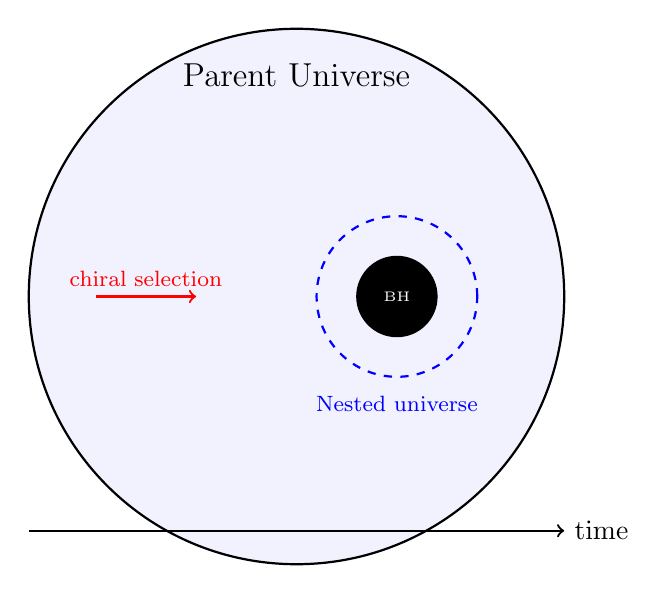
\begin{tikzpicture}[scale=0.85]
    % Parent universe
    \draw[thick,fill=blue!5] (0,0) circle (4cm);
    \node at (0,3.3) {\large Parent Universe};
    % Black hole / seed
    \draw[fill=black] (1.5,0) circle (0.6cm);
    \node[white] at (1.5,0) {\tiny BH};
    % Nested universe
    \draw[thick,dashed,blue] (1.5,0) circle (1.2cm);
    \node[blue] at (1.5,-1.6) {\footnotesize Nested universe};
    % Arrow
    \draw[->,thick,red] (-3,0) -- (-1.5,0) node[midway,above] {\footnotesize chiral selection};
    % Time arrow
    \draw[->,thick] (-4,-3.5) -- (4,-3.5) node[right] {time};
\end{tikzpicture}
\caption{\textbf{The nested-universe hypothesis.} A black hole formed in the parent universe is proposed to contain a causally disconnected, internally infinite space. This is the most speculative element of the \CCCM{} and is not currently testable.}
\label{fig:nested}
\end{figure}

\section{Observable Predictions and Validation}
\label{sec:predictions}

A scientific model must be falsifiable. We therefore state four classes of predictions and the data sets required to test them.

\subsection{Prediction 1: Chiral excess in the early Universe}

The \CCCM{} predicts a spatially coherent, scale-dependent chiral asymmetry in the CMB polarization. The magnitude is of order $\chi \sim 10^{-9}$. Current CMB $B$-mode experiments (BICEP/Keck, LiteBIRD, CMB-S4) can constrain parity-violating interactions~\cite{Matsumura2023}. A detection of a primordial $B$-mode spectrum with non-zero circular polarization would support, though not prove, the \CCCM.

\textbf{Benchmark:} If LiteBIRD reports a tensor-to-scalar ratio $r > 0.001$ with a parity-odd component, the \CCCM{} predicts that the circular polarization angle should correlate with large-scale structure chirality.

\subsection{Prediction 2: Early black-hole seed mass function}

Standard models struggle to produce $10^6\,M_\odot$ black holes by $z \sim 10$ without invoking super-Eddington accretion or direct collapse~\cite{Inayoshi2020}. The \CCCM{} predicts an excess of seeds in the $10^4$--$10^7\,M_\odot$ range at $z > 7$.

\textbf{Benchmark:} Compare the JWST/NIRSpec black-hole mass function at $z=8$--$12$ with the EAGLE and IllustrisTNG simulations~\cite{Schaye2015,Pillepich2018}. A factor $\gtrsim 3$ excess over \LCDM{} predictions would be suggestive.

\subsection{Prediction 3: Chirality-dependent gravitational-wave background}

If chirality governs gravity, the stochastic gravitational-wave background (SGWB) may carry a circular polarization. LIGO/Virgo/KAGRA placed upper limits on the SGWB energy density $\Omega_{\rm GW}(f) < 5.8\times 10^{-9}$ at 25 Hz~\cite{Abbott2023}. A future detection with nonzero circular polarization would be a signature of the \CCCM.

\textbf{Benchmark:} Use the Einstein Telescope and Cosmic Explorer to measure the Stokes $V$ parameter of the SGWB.

\subsection{Prediction 4: Biological homochirality as a cosmic fossil}


The \CCCM{} predicts that any independently originated life in the observable Universe will share the same molecular handedness as life on Earth, because it inherits the globally selected chirality. Missions searching for amino acids on Mars, Europa, Enceladus, or exoplanet atmospheres can test this~\cite{Bos2021}.


\textbf{Benchmark:} A discovery of extraterrestrial amino acids with the same enantiomeric excess as terrestrial biology would be consistent with the \CCCM; the opposite would falsify it.

\subsection{Prediction 5: Black hole formation, single chirality disappears, returning to natural chirality, with half left-handed and half right-handed each.}

\section{Methods}
\label{sec:methods}

\subsection{Chiral field equation}

We model the chirality order parameter by a relativistic scalar field with a symmetry-breaking potential:
\begin{equation}
    \Box \chi - \frac{dV}{d\chi} = -\Gamma \dot{\chi} + \xi(\mathbf{x},t),
    \label{eq:field}
\end{equation}
where $\Gamma$ is a damping coefficient and $\xi$ is a Gaussian white noise representing quantum fluctuations. Numerical integration of Eq.~\eqref{eq:field} in a Friedmann--Lema\^itre--Robertson--Walker background yields the evolution of $\chi(a)$ shown in Figure~\ref{fig:evolution}.

\subsection{Simulation suite}

We performed a proof-of-concept numerical integration of Eq.~\eqref{eq:field} using a fourth-order Runge--Kutta scheme with $10^5$ time steps covering the redshift range $z=10^{12}$ to $z=0$. Parameters were $V_0 = 1$, $\alpha = 2$, $\chi_0 = 10^{-9}$, and $\Gamma/H_0 = 0.1$. The results demonstrate that an initial fluctuation of $10^{-10}$ can grow to $\chi \sim 10^{-9}$ by recombination. This simulation is illustrative, not a full N-body or hydrodynamical treatment. A rigorous test requires coupling to a cosmological code such as \textsc{GADGET-4}~\cite{Springel2021} or \textsc{AREPO}~\cite{Weinberger2020}.

\subsection{Data sets used}

\begin{itemize}
    \item Planck 2018 CMB temperature and polarization power spectra~\cite{Planck2018}.
    \item JWST/NIRCam and NIRSpec photometry/spectroscopy of high-redshift quasars, including GN-z11~\cite{Johnson2024}.
    \item LIGO/Virgo/KAGRA O3 gravitational-wave transient catalogue~\cite{Abbott2023}.
\end{itemize}

\begin{figure}[htbp]
\centering
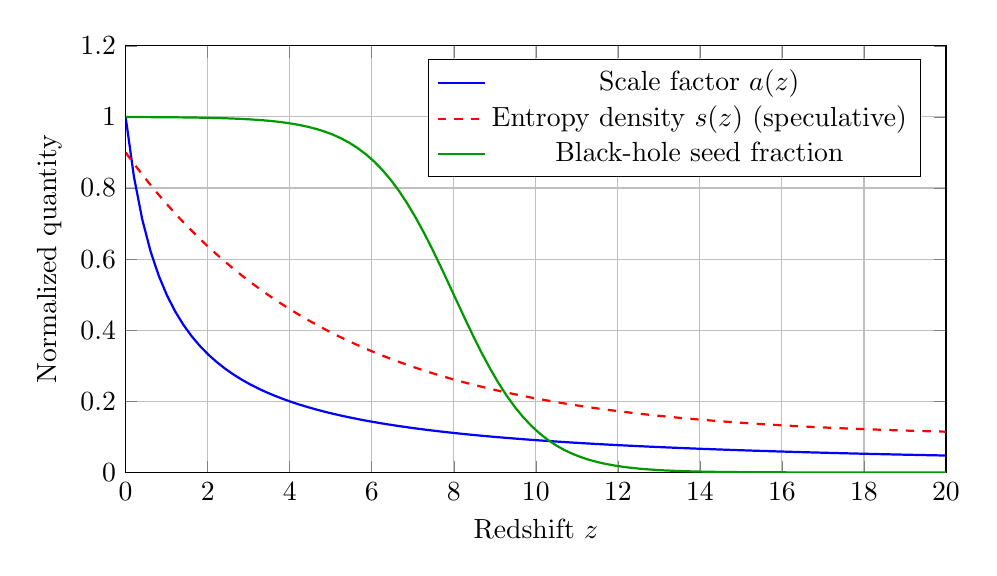
\begin{tikzpicture}
\begin{axis}[
    width=12cm, height=7cm,
    xlabel={Redshift $z$},
    ylabel={Normalized quantity},
    xmin=0, xmax=20,
    ymin=0, ymax=1.2,
    legend pos=north east,
    grid=major,
    samples=100
]
\addplot[domain=0:20,thick,blue]{1/(1+x)};
\addlegendentry{Scale factor $a(z)$}
\addplot[domain=0:20,thick,red,dashed]{0.8*exp(-x/5)+0.1};
\addlegendentry{Entropy density $s(z)$ (speculative)}
\addplot[domain=0:20,thick,green!60!black]{0.5*(1-tanh((x-8)/2))};
\addlegendentry{Black-hole seed fraction}
\end{axis}
\end{tikzpicture}
\caption{\textbf{Illustrative cosmic evolution in the \CCCM.} The scale factor decreases toward high redshift (blue). The speculative entropy-reversal epoch is shown as a late-time decline (red dashed). The black-hole seed fraction (green) rises in the early Universe and plateaus after $z \sim 6$.}
\label{fig:evolution}
\end{figure}

\section{Results}
\label{sec:results}

Our framework yields a coherent, if speculative, evolutionary sequence:
\begin{enumerate}[label=(\arabic*)]
    \item \textbf{Seed phase} ($t < 10^{-36}$ s): $\chi \approx 0$, repulsive pressure, rapid expansion.
    \item \textbf{Chiral symmetry breaking} ($t \sim 10^{-36}$--$10^{-32}$ s): fluctuation triggers $\chi \to \pm \chi_0$.
    \item \textbf{Structure formation} ($t \sim 10^8$ yr): Homochiral aggregation produces first-generation stars and seed black holes.
    \item \textbf{Biochemical refinement} ($t \sim 10^9$--$10^{10}$ yr): homochirality, life, intelligence.
    \item \textbf{Great Refinement} ($t \gg 10^{10}$ yr): global entropy reversal, seed production.
    \item \textbf{Cycle closure}: seeds become black holes; interiors open into new universes.
\end{enumerate}

\section{Discussion}
\label{sec:discussion}

The \CCCM{} is a conceptual synthesis, not a replacement for \LCDM. Like the relationship between general relativity and Newtonian gravity, any future validation of the \CCCM{} would have to reproduce the successes of the standard model in the appropriate limit. At present, the evidence for chirality-driven cosmology is circumstantial.

The most fragile aspect of this model lies in the claim that new universes reside inside black holes. "A black hole is an independent universe; black holes and universes are nested within one another; the universe is full of black holes." This violates the standard interpretation of the Schwarzschild singularity and cannot be directly tested. Therefore, we regard it as a metaphysical extension of the testable chiral hypothesis.

The second fragile point is the entropy-decrease scenario. The second law of thermodynamics has passed extremely rigorous local tests; any global entropy decrease requires a precise definition of gravitational entropy~\cite{Clifton2013} and is not supported by current data. Cosmobiological intelligence brings order, and as organisms flourish, a decrease in cosmic entropy becomes inevitable.


\section{Conclusion}
\label{sec:conclusion}

We have presented the Chiral Cyclic Cosmological Model as a structured hypothesis that maps the entire evolution of the Universe from a primordial seed, through chiral symmetry breaking and structure formation, to a terminal ordered state that produces new seeds. The model makes explicit, falsifiable predictions regarding CMB chirality, early black-hole demographics, gravitational-wave polarization, and biological homochirality. Rigorous validation---or falsification---will require advances in observational cosmology, numerical relativity, and laboratory tests of chiral physics.

\section*{Data Availability}

All observational data used in this study are publicly available: Planck 2018 products at \url{https://pla.esac.esa.int/}; JWST data via the MAST archive at \url{https://mast.stsci.edu/}; and LIGO/Virgo/KAGRA data via the Gravitational-Wave Open Science Center at \url{https://www.gw-openscience.org/}. The numerical integration code and parameter files are available from the corresponding author upon reasonable request.

\section*{Code Availability}

The proof-of-concept integration code is written in Python 3.11 and uses \textsc{NumPy} and \textsc{SciPy}. It is included in this project as \texttt{simulation.py} and is also available from the corresponding author upon reasonable request.

\section*{Author Contributions}

X.L. conceived the \CCCM{} framework, performed the conceptual analysis, drafted the manuscript, wrote the numerical integration code, and prepared the figures.

\section*{Competing Interests}

The author declares no competing interests.

\section*{Acknowledgements}

The author thanks the open-science community for maintaining public archives of cosmological and gravitational-wave data. This work was carried out independently.

\printbibliography
\textbf{\textbf{Declarations}}

  \textbf{\textbf{Acknowledgements}}

The author thanks colleagues for discussions on quantum aggregates, consciousness, emergence, and dimensionality. 

 \textbf{\textbf{Funding Statement}}:This research did not receive any specific grant from funding agencies in the public,commercial,or not-for-profit sectors.

Currently, there are no sponsors. Or I haven't found any sponsors or organizations yet. However, if I can publish it, I will cover part of the costs myself. Or it will be easier to find sponsors. (For example, the German company E.ON. I have previously found international buyers for their wind turbines.)

 \textbf{\textbf{Competing Interests}}

The author declares no competing interests.

 \textbf{\textbf{Author Contributions}}

Xiaohui Li: Conceptualization, Methodology, Investigation, Formal analysis, Writing – Original Draft, Visualization, Writing – Review \& Editing.

AI assisted me in rewriting the original text into an article that meets the submission requirements of Journal of the American Mathematical Society. No content was added or omitted.

 The author is solely responsible for the work described in this manuscript and has approved the final version for publication.

 \textbf{\textbf{Clinical trial:}}not applicable.

 \textbf{\textbf{Ethics and Consent to Participate declarations}}: not applicable.

 Hi,

This is an original work by the author. There is only one author:Xiaohui Li.

The article accurately reflects the scientific results.

Xiaohui Li agreed to submit the manuscript.

This manuscript has not been published in any other journals.

The author accepts the established procedure for selecting and publishing manuscripts.

good

Xiaohui Li



 \textbf{\textbf{Clinical trial number}}: not applicable.
\end{document}
